\section{Softwarearchitektur}

\subsection{Strategie}


\subsection{Erkundung der Karte} \label{erkundungDerKarte}

\subsubsection{Kreisförmige Karte} ~\\

Hier geht es darum, dass die Karte keinen Rand hat. \\
Kurz beschreiben, dass wir zu Beginn eine begrenzte Karte hatten und dann eine offene Karte

\subsection{Entscheidungsverhalten der Agenten}

\subsubsection{Rollen} ~\\
Die Rollen werden in der Serverkonfiguration vorgegeben. In den Turnieren standen fünf Rollen bereit: default, worker, constructor, explorer und digger. \\
Die Rollen haben verschiedene Aktionen, welche sie ausführen dürfen. Zu Beginn haben alle Agenten die \textit{default}-Rolle inne. Diese enthält alle Standardaktionen wie \textit{move, rotate, skip, adopt, detach und clear}. Um nach verschiedenen Dingen suchen zu können, benötigen die Agenten die Rolle \textit{explorer}. Mit diesen kann ein \textit{survey} nach einem Dispenser gemacht werden. Sobald die Agenten die Aufgabe bekommen einen Block abzuholen, müssen sie in die Rolle \textit{worker} wechseln. Damit können sie Blocke aufnehmen, sich mit anderen Agenten verbinden und auch die Aufgaben abgeben. 
Die Besonderheit ist, dass alle Rollen die Aktionen der default-Rolle erben. Die Standardaktionen besitzen somit alle anderen Rollen ebenfalls.

Die Rolle \textit{constructor} und \textit{digger} hat die Gruppe nicht weiter verfolgt, da diese für unsere Strategie nicht notwendig war. 

\subsubsection{Aufgaben} ~\\
NextTaskPlanner umgesetzt

Liste der Pläne: 
exploreMap,\\
goToDispenser,\\
goToGoalzone,\\
goToRolezone,\\
solveTask,\\
surveyDispenser,\\
surveyGoalZone,\\
surveyRoleZone,\\
surveyRandom,\\
connectToAgent,\\
discoverMapSize,\\
cleanMap,\\

\subsubsection{Wegfindung} \label{kap:wegfindung} ~\\
Random \newline
Spirale \newline
Manhattan \newline
A*

\subsubsection{Gruppenbildung} \label{kap:Gruppenbildung} ~\\

Gruppenbildung

\subsection{Globale und lokale Sicht}
Die Sicht der Agenten können in eine globale und eine lokalen Sicht unterschieden werden. Die globale Sicht besteht aus einer gespeicherten Karte pro Agent, die sich durch die Bewegungen des Agenten auf der Karte erweitert. Hier werden die verschiedenen Dinge wie Dispenser, Blöcke oder Zonen gespeichert. Sobald sich die Agenten in Gruppen finden, werden die Karten synchronisiert. Eine genauere Erklärung zu den Karten befindet sich im Kapitel \textit{\ref{erkundungDerKarte}}.\\

Die lokale Sicht des Agenten ist auf eine festgelegte Größe beschränkt. Die Sichtweite des Agenten wird in der Serverkonfiguration festgelegt. Bei einer Sichtweite von 5 sieht der Agent 5 Kästchen nach links, rechts, oben und unten, wie in Abbildung \ref{fig:agentensicht} dargestellt.
\begin{figure}
	\centering
	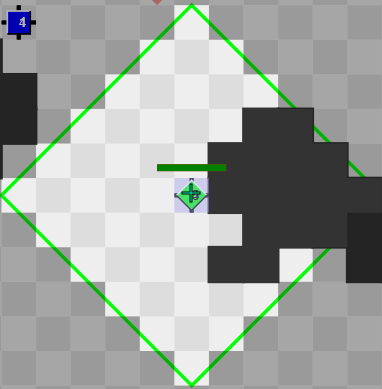
\includegraphics[width=150px]{bilder/agentensicht}
	\caption{Sicht des Agenten}
	\label{fig:agentensicht}
\end{figure}

Im ersten Schritt ermittelt der Agent einen möglichen Weg, wie er zu seinem Ziel gelangt. Hierfür wird der entsprechende Wegalgorithmus verwendet, welcher in Kapitel \textit{\ref{kap:wegfindung}]} genauer erläutert wird. Sobald der Weg ermittelt wurde und bevor ein Schritt des Weges beschritten wird, prüft der Agent auf Aktionen, welche vorher ausgeführt werden müssen. Diese Aktionen können einen Rollenwechseln beinhalten, ungenutzte Blöcke fallen lassen, einen Block vom Dispenser anfordern oder einen Block aufnehmen, eine Aufgabe in der Endzone abgeben oder sich mit einem anderen Agenten verbinden. Diese Aktionen sind Momentaufnahmen, die der Agent ausführen muss, bevor er zu einem neuen Ziel geht. Wenn keine dieser Aktionen passt, wird der Agent den Weg zu seinem Ziel gehen. Hier kommt nochmals eine Entscheidungsmöglichkeit für den Agenten in Frage. Ist der nächste Schritt frei und ich kann den Weg gehen, dann geht er diesen. Sollte aber beispielsweise ein Block in der Richtung sein, in die der Agent gehen möchte, so muss er diesen zunächst zerstören. Wenn ein Agent in der Richtung steht, so wird ein Weg um diesen Agenten herum erstellt. In Abbildung \ref{fig:agentensicht} wäre der Weg in Richtung Westen durch einen Block gehindert, sodass er diesen zunächst zerstören muss, bevor er in diese Richtung gehen kann. 

Zusammengefasst muss der Agent in jedem Schritt entscheiden, ob es eine Aktion gibt, die gerade notwendig ist, wie einen Block aufzunehmen oder ob der Schritt, den er gehen möchte, möglich ist.  

\subsection{Synchronisation und Kommunikation}
Die Kommunikation der Agenten funktioniert, sobald sie sich in einer Gruppe befinden. Die Synchronisation der Gruppen ist in Kapitel \textit{\ref{kap:Gruppenbildung}} genauer beschrieben. Für die Kommunikation wurde eine Schnittstelle entwickelt, welche die Nachricht, den Senderagenten und den Empfängeragenten in einer Nachrichtenbox bereithält. Stehen zwei Agenten um einen Dispenser und beide möchten einen Block anfordern, so wird der Agent zunächst prüfen, ob eine Nachricht für ihn vorliegt. Ist dies nicht der Fall, untersucht der Agent, ob andere Agenten in der nähe des Dispensers stehen. Wenn die Prüfung erfolgreich ist, so wird er eine Nachricht an den Agenten senden und dieser wird dann warten, bis der Dispenser frei ist. Er selbst stellt eine Anfrage an den Dispenser und nimmt den Block dann auf. 